\documentclass[11pt,a4paper]{book}
%%%Preamble
\title{Latex: La referencia completa e introducción}
\author{j3w1}
\date{29 de diciembre de 2019}

%%% Packages
\usepackage[T1]{fontenc}
\usepackage[utf8]{inputenc}
\usepackage[spanish]{babel}
\usepackage{hyperref}
\usepackage{listings}
\usepackage{pdfpages}
\usepackage{pagecolor}
\usepackage{xcolor}

\color{white}
\pagecolor{black}
%%% Document
\begin{document}

	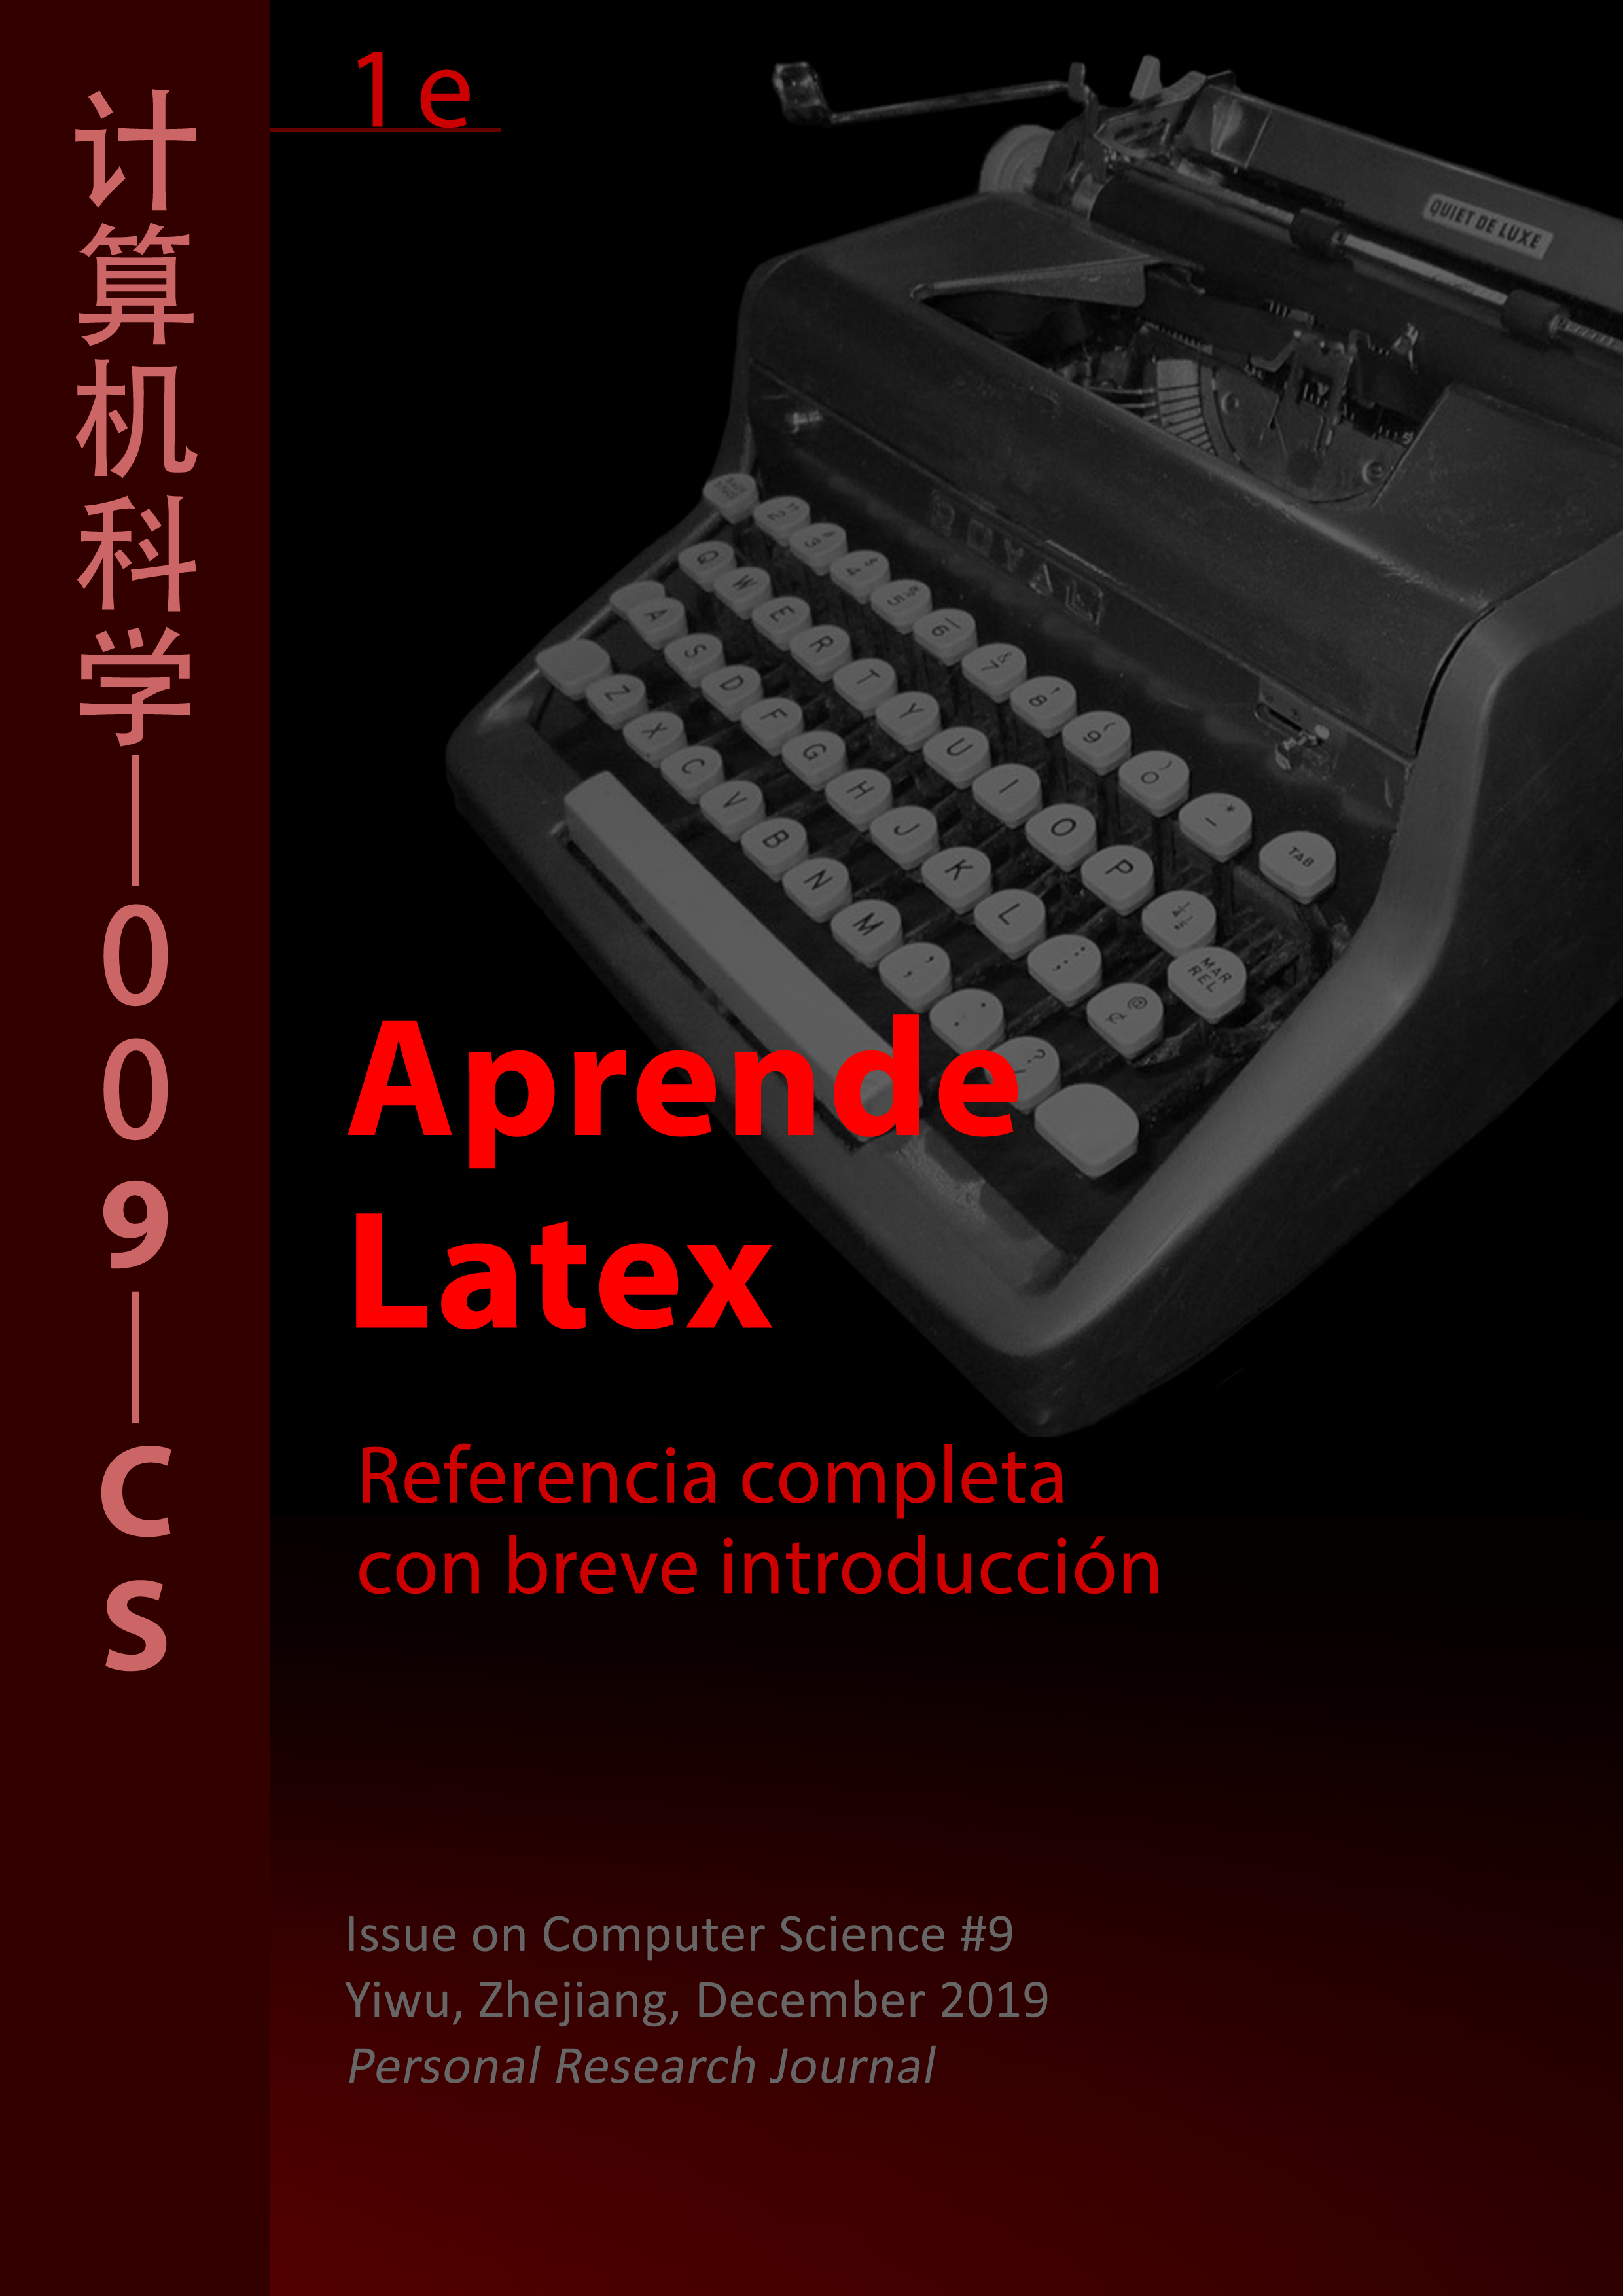
\includepdf{resources/Cover.pdf}
	\thispagestyle{plain}
    \maketitle

    \section*{Prefacio}\label{sec:preface}
    \noindent Por cada vez que usé un procesador de textos, desearía haber conocido cuanto más antes esta plataforma de tipografía, \LaTeX\ ha probado ser una verdadera alternativa para aquellos programadores o entusiastas de la escritura académica.
    Si bien, la plataforma tiene características de ser un \emph{framework} completo de literatura científica, libre de distracciones; \LaTeX\ ha sido, desde un principio, planeado por una persona con técnica y desarrollado por ingenieros alrededor de todo el mundo, a modo de \emph{software} libre, con el puro objetivo de implementar un lenguaje de programación, enfocados en el programador-científico que despliegue sus archivos académicos de igual forma en que elabora sus paquetes de código o \emph{APIs}. \TeX\ y \LaTeX\ han probado ser aquel entorno amigable para el programador que necesita de la única definitiva herramienta para editar, organizar, compilar los \emph{papers} que documentarán los experimentos y que mantendrá un registro de sus experiencias recolectados en la manera más purista, elegante y legible posible.

    En este informe (al igual que planeo hacer con todos mis \emph{journals}) registraré cada aprendizaje, sintaxis, reseña, comentario, idea, experiencia, una que otra línea de código y todo aquello que haya servido como ruta de aprendizaje a esta maravillosa herramienta.
    La intención de todo esto, desde el despliegue del repositorio (\href{https://github.com/1w3j/CS}{1w3j/CS.git}), hasta la constante manutención del proyecto, es simplemente conllevar mientras dure, un tipo de diario que sirva de rápido apunte, futura redacción, versátil referencia para mis propios intereses y de encontrar la información necesitada en el momento que se requiera.

    Este documento, en el momento en que estoy escribiendo este párrafo \footnote{30 de Diciembre de 2019 5:28 p.m.} es en sí una gran sola práctica y ejercicio de la ruta hacia \LaTeX, además de, mi primer desarrollo escrito.
    En momentos oportunos, se irán añadiendo contenidos que espero aporte valor en algún futuro como información-referencia.
    Me interesé tanto en el tema, que nada más espero el camino se duradero y lleno de aprendizaje.
    
    \tableofcontents

	\part[Fundamentos]{FUNDAMENTOS}

		\chapter{Introducción}\label{ch:intro}
			Aquí llenar la introducción
			\section{Qué es \LaTeX?}\label{sec:what-is-latex}
				\noindent Simple pregunta y simple respuesta, \LaTeX\ es un programa de \emph{tipografeado}\footnote{Se refiere a la función que cumplen aquellas máquinas de escribir de décadas posteriores} y una extensión del programa original \TeX\ creado por Donald Knuth.

				A comparación con los procesadores de texto, en \LaTeX\ tenemos todas las operaciones y funcionalidades empaquetados en una sola aplicación.
				\mbox{La ventaja} es que a \TeX\ solo le importa el contenido que va \emph{tipeado} en los archivos de texto.
				Entonces, podemos utilizar piezas de \emph{software} tan predeterminadas como un editor de texto: \emph{Vim, emacs, Notepad++}, subir los archivos \emph{*.tex} a un repositorio, organizar \emph{agile} con tu equipo de trabajo y distribuir la documentación entre los programadores para su posterior implementación.
				Las posibilidades son infinitas, debido que, al componer \LaTeX, básicamente estamos transcribiendo nuestro contenido en un archivo de texto plano para luego compilarlo.
				Después podemos abrirlo en un visualizador de documentos o imprimir el contenido usando un \emph{driver} de impresión.

				\TeX\ es de raíz un lenguaje de programación, al igual que \emph{Python}, \TeX\ tiene su propio sistema de paquetes.
				Programadores pueden crear sus propios, cada vez más personas dedicadas contribuyen con el proyecto e incluso podemos distribuir nuestro código fuente en modo de paquetes, a otros usuarios, así es, \LaTeX\ es \TeX\ con una gran colección de funcionalidades pensadas en la redacción de contenido técnico lo cual hace de \TeX\ la plataforma de desarrollo de documentos académicos-científicos por defecto.

				\subsection{Un pequeño ejemplo}\label{subsec:little-example}
					Note the `difference` in 'right' and 'left'' quotes in \lq single quotes\rq\ and \lq\lq double quotes\rq\rq.
					\indent\lstinputlisting[language=TeX]{listings/list1.tex}

			\section{¿Por qué \LaTeX?}\label{subsec:¿por-qué-latex?}

		\section{Primeros pasos}\label{sec:first-steps}


\end{document}
